% Options for packages loaded elsewhere
\PassOptionsToPackage{unicode}{hyperref}
\PassOptionsToPackage{hyphens}{url}
%
\documentclass[
]{book}
\usepackage{lmodern}
\usepackage{amssymb,amsmath}
\usepackage{ifxetex,ifluatex}
\ifnum 0\ifxetex 1\fi\ifluatex 1\fi=0 % if pdftex
  \usepackage[T1]{fontenc}
  \usepackage[utf8]{inputenc}
  \usepackage{textcomp} % provide euro and other symbols
\else % if luatex or xetex
  \usepackage{unicode-math}
  \defaultfontfeatures{Scale=MatchLowercase}
  \defaultfontfeatures[\rmfamily]{Ligatures=TeX,Scale=1}
\fi
% Use upquote if available, for straight quotes in verbatim environments
\IfFileExists{upquote.sty}{\usepackage{upquote}}{}
\IfFileExists{microtype.sty}{% use microtype if available
  \usepackage[]{microtype}
  \UseMicrotypeSet[protrusion]{basicmath} % disable protrusion for tt fonts
}{}
\makeatletter
\@ifundefined{KOMAClassName}{% if non-KOMA class
  \IfFileExists{parskip.sty}{%
    \usepackage{parskip}
  }{% else
    \setlength{\parindent}{0pt}
    \setlength{\parskip}{6pt plus 2pt minus 1pt}}
}{% if KOMA class
  \KOMAoptions{parskip=half}}
\makeatother
\usepackage{xcolor}
\IfFileExists{xurl.sty}{\usepackage{xurl}}{} % add URL line breaks if available
\IfFileExists{bookmark.sty}{\usepackage{bookmark}}{\usepackage{hyperref}}
\hypersetup{
  pdftitle={Knowledge Pool},
  pdfauthor={DAVeMoS team, Institute for Transport Studies (IVe), University of Natural Resources and Life Sciences in Vienna},
  hidelinks,
  pdfcreator={LaTeX via pandoc}}
\urlstyle{same} % disable monospaced font for URLs
\usepackage{longtable,booktabs}
% Correct order of tables after \paragraph or \subparagraph
\usepackage{etoolbox}
\makeatletter
\patchcmd\longtable{\par}{\if@noskipsec\mbox{}\fi\par}{}{}
\makeatother
% Allow footnotes in longtable head/foot
\IfFileExists{footnotehyper.sty}{\usepackage{footnotehyper}}{\usepackage{footnote}}
\makesavenoteenv{longtable}
\usepackage{graphicx,grffile}
\makeatletter
\def\maxwidth{\ifdim\Gin@nat@width>\linewidth\linewidth\else\Gin@nat@width\fi}
\def\maxheight{\ifdim\Gin@nat@height>\textheight\textheight\else\Gin@nat@height\fi}
\makeatother
% Scale images if necessary, so that they will not overflow the page
% margins by default, and it is still possible to overwrite the defaults
% using explicit options in \includegraphics[width, height, ...]{}
\setkeys{Gin}{width=\maxwidth,height=\maxheight,keepaspectratio}
% Set default figure placement to htbp
\makeatletter
\def\fps@figure{htbp}
\makeatother
\setlength{\emergencystretch}{3em} % prevent overfull lines
\providecommand{\tightlist}{%
  \setlength{\itemsep}{0pt}\setlength{\parskip}{0pt}}
\setcounter{secnumdepth}{5}
\usepackage{booktabs}
\usepackage{amsthm}
\makeatletter
\def\thm@space@setup{%
  \thm@preskip=8pt plus 2pt minus 4pt
  \thm@postskip=\thm@preskip
}
\makeatother
\usepackage[]{natbib}
\bibliographystyle{apalike}

\title{Knowledge Pool}
\author{DAVeMoS team, Institute for Transport Studies (IVe), University of Natural Resources and Life Sciences in Vienna}
\date{2021-11-15}

\begin{document}
\maketitle

{
\setcounter{tocdepth}{1}
\tableofcontents
}
\hypertarget{welcome}{%
\chapter{Welcome}\label{welcome}}

\hypertarget{intro}{%
\chapter{Einleitung}\label{intro}}

Diese Arbeit sammelt und definiert wesentliche Konzepte im Zusammenhang mit der Automatisierung und Digitalisierung des Verkehrssystems zusammen mit der Beschreibung ihrer Auswirkungen, sowohl negativ als auch positiv auf \textbf{individueller}, \textbf{systemischer} und \textbf{wirtschaftlicher Ebene}. Dieser Knowledge pool wird durch die Tatsache angetrieben, dass Automatisierung und Digitalisierung schnell voranschreiten, wenn auch nicht gleichmäßig in allen Bereichen im Verkehrskontext. Um das Spektrum der Möglichkeiten zu verstehen, die sie mit sich bringen, ist es daher notwendig, die Schlüsselkonzepte zu erklären, ihren Entwicklungsstand und ihre derzeitige Marktdurchdringung aufzuzeigen und schließlich ihre Auswirkungen auf verschiedenen Ebenen zu bewerten. Angesichts dieses Ansatzes enthält jedes Thema die folgenden \textbf{Definition} des Phänomens,
\textbf{Wichtige Interessensgruppen}, die für die jeweilige technologische Entwicklung verantwortlich und von ihr betroffen sind. Dann folgen zwei Unterabschnitte zum \textbf{aktuellen Stand der Forschung und Praxis}. Der erste Abschnitt fasst die neuesten Forschungsergebnisse zu einem bestimmten Thema zusammen, während der zweite Abschnitt den aktuellen Stand der Umsetzung einer bestimmten Technologie in der realen Welt erläutert. Der Abschnitt ``\textbf{Relevante Initiativen in Österreich}'' beschreibt die führenden Initiativen zu einem bestimmten Thema und das Potenzial für österreichische Akteure. Darüber hinaus bieten wir eine zusammenfassende Tabelle über die Auswirkungen des Konzepts auf ausgewählte \textbf{Ziele für nachhaltige Entwicklung} (SDGs). Um ein objektives Maß für den Entwicklungsstand der Technologie in den einzelnen Themenbereichen zu erhalten, haben wir außerdem die sogenannte \textbf{Technology Readiness Scale} (Williamson \& Beasley, 2011) wie unten beschrieben, integriert:

\begin{figure}
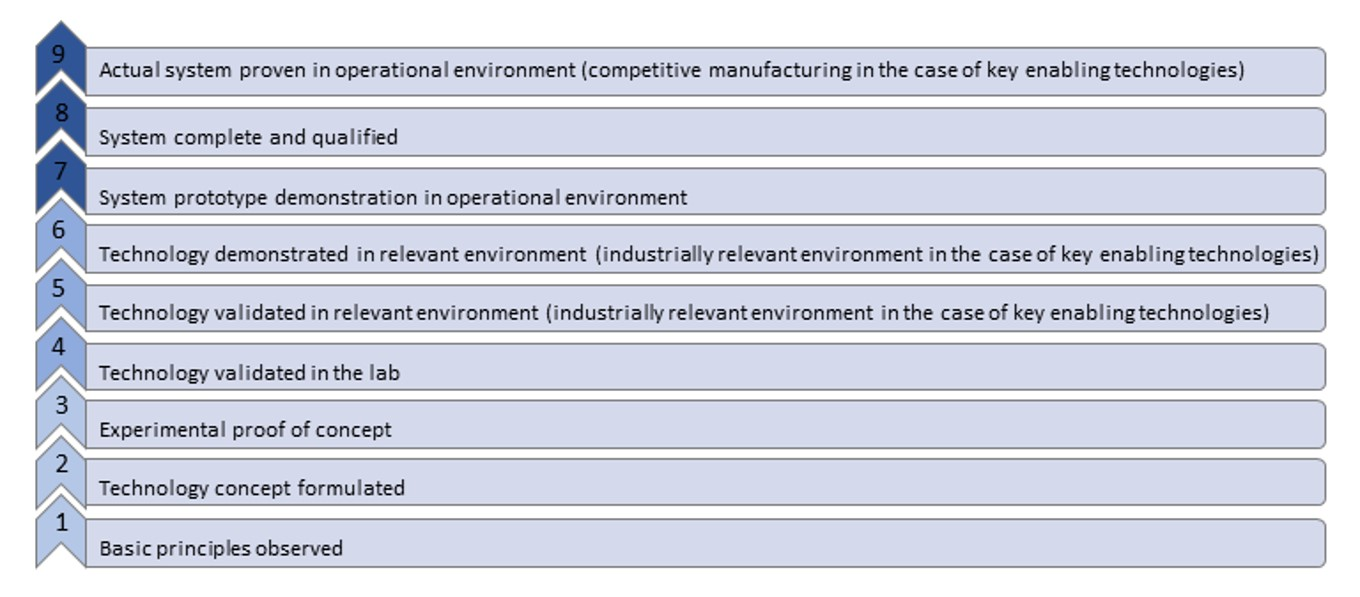
\includegraphics[width=0.8\linewidth]{image/TRL_cropped} \caption{Skala der technologischen Bereitschaft.}\label{fig:unnamed-chunk-1}
\end{figure}

Darüber hinaus bewerten wir die Bereitschaft einer bestimmten Technologie, in der Gesellschaft akzeptiert zu werden, und wie gut sie zum Gemeinwohl beiträgt, indem wir die \textbf{Skala der gesellschaftlichen Bereitschaft} verwenden (McCulloch, 2019):

\begin{figure}
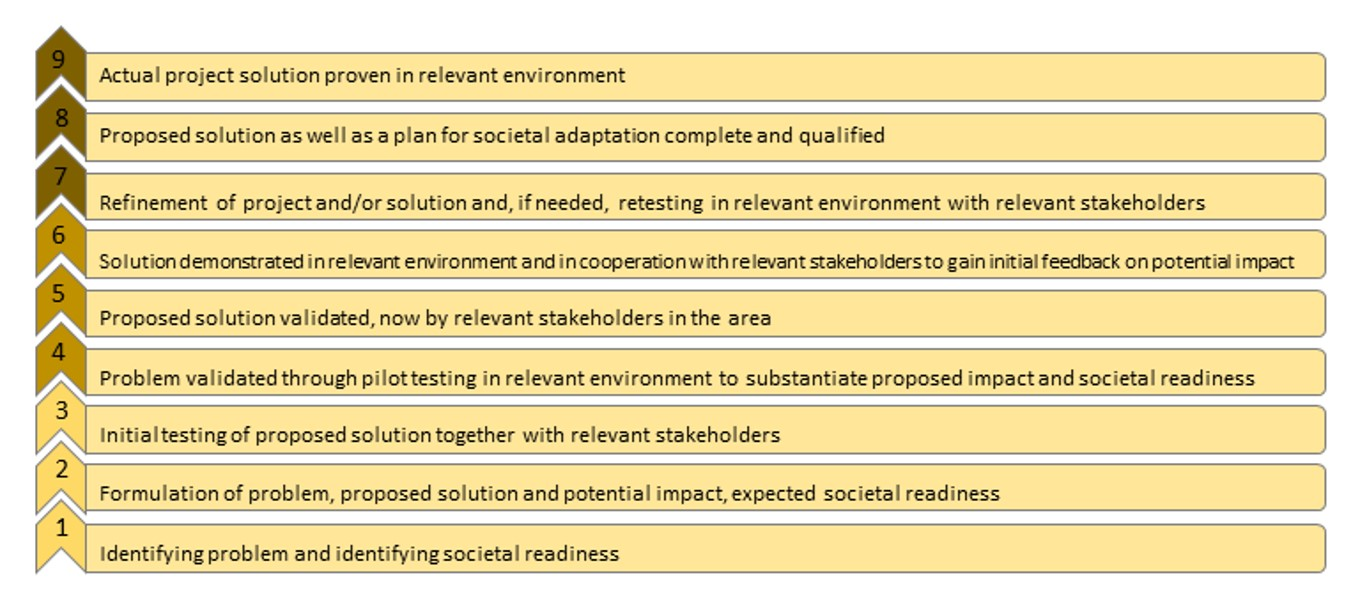
\includegraphics[width=0.8\linewidth]{image/SRL_cropped} \caption{Skala fuer die gesellschaftliche Bereitschaft.}\label{fig:unnamed-chunk-2}
\end{figure}

Abschließend finden Sie eine Liste \textbf{offener Fragen} und \textbf{Links zu weiteren Quellen} zu diesem Thema.

\textbf{Referenzen}

\begin{itemize}
\tightlist
\item
  Williamson, R., \& Beasley, J. (2011). \emph{Automotive technology and manufacturing readiness levels: a guide to recognised stages of development within the automotive industry}. URN11/672.
\item
  McCulloch, S. (2019). Social Acceptance And Societal Readiness Levels. \emph{DecarboN8}. Available at: \url{https://decarbon8.org.uk/social-acceptance-and-societal-readiness-levels/\#:~:text=Societal\%20readiness\%20refers\%20to\%20the,contributes\%20to\%20the\%20public\%20good.} {[}Accessed: 21 January 2021{]}.
\end{itemize}

  \bibliography{book.bib,packages.bib}

\end{document}
